\section{\texstud}
\texstud  ist ein plattformunabhängiger Editor, um komfortabel \LaTeX -Dokumente zu
erstellen. Es ist einfach zu bedienen und richtet sich vor allem an die Zielgruppe \LaTeX -Einsteiger.
Im Vergleich zu anderen \LaTeX -Editoren beweist sich \texstud als eines der
Programme mit den umfangreichsten Funktionen. Zudem gibt es sowohl Versionen für
Linux, als auch für Windows und Mac OS. Durch die Plattformunabhängigkeit können
eine Reihe an externen Programmen integriert werden, darunter Rechtschreibüberprüfungen in verschiedenen Sprachen. Zudem bietet es eine rundum
Hilfestellung, das Aufspüren und Beseitigen von Fehlern und eine sofortige Vorschau.

\subsection{Benutzeroberfläche}
Die Oberfläche besteht aus einer Symbolleiste, einem Editor und einer Konsole, die
zusammengefasst in einem großen Hauptfenster erscheinen. Dieses Konzept verleiht der
Software ein recht homogenes Aussehen, wirkt aber unter bestimmten Umständen – etwa
auf kleinen Bildschirmen – schnell unübersichtlich. Neben Menü und Werkzeugleiste finden sich im Fenster mehrere Ein- und Ausgabebereiche. Die Werkzeugleisten lassen sich mit der Maus verschieben; einzelne Menüs können über den Konfigurationsdialog unter Menüs ein- oder ausgeblendet werden. \\\\
\begin{minipage}[h]{\textwidth}
	\centering	
	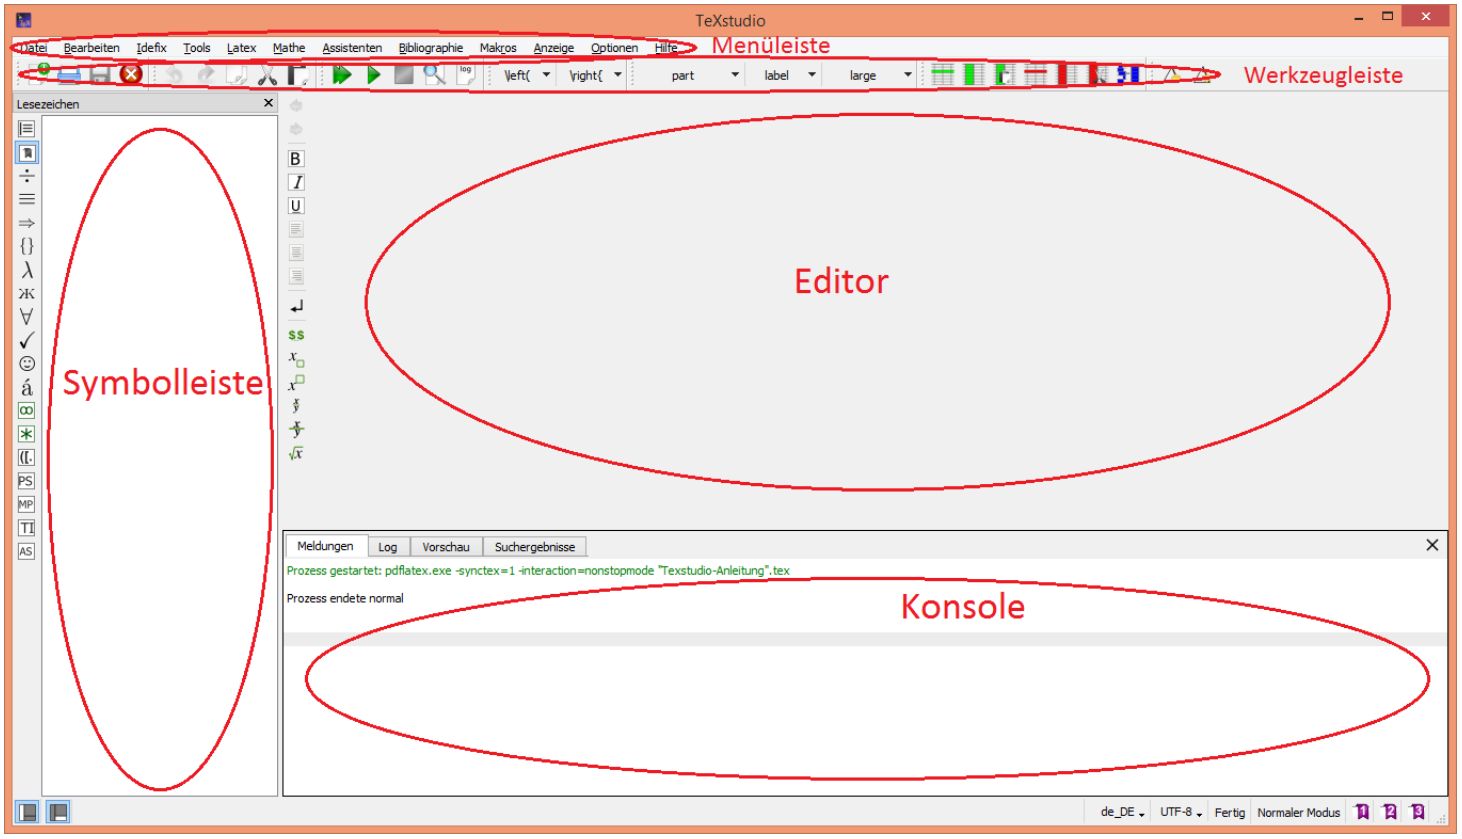
\includegraphics[width=\textwidth]{images/texstudiogui}
	\captionof{figure}{Benutzeroberfläche \texstud}
	\label{fig:gui}
\end{minipage}\clearpage
\begin{itemize}
	\item \textbf{Editor:} Hier können die \LaTeX -Dokumente bearbeitet werden.% Beim Kompilieren eines Dokuments kann zusätzlich noch ein PDF-Viewer eingeblendet werden.
	\item	\textbf{Konsole:} Hier werden etwaige Fehlermeldungen beim Kompilieren ausgeben.
	\item \textbf{Symbolleiste:} Hier wird die interne Hierarchie des aktuell bearbeiteten Files angezeigt. \\
\end{itemize}

Das Aussehen des Editors kann unter \textit{Optionen > \texstud konfigurieren}
im Detail eingestellt werden. Unter \textit{Editor} legt man das grundlegende Verhalten fest. Im Dialog \textit{Erweiterter Editor} die Feinheiten, wie Breite des Tabulators, die Suchfunktion oder den automatischen Zeilenumbruch.

%\subsection{Neues Dokument hinzufügen}\vspace{-10pt}
%Um ein neues Dokument zu erstellen drücken sie auf folgendes Icon 
\includegraphics[width=18pt]{images/newfile}. Danach öffnet sich ein neues Dokument. \\
%\aufgabe{Neues Dokument erstellen}{Erstelle ein neues Dokument \textit{\glqq Tutorial.tex\grqq{}} und speichere es im Unterordner \textit{\glqq sections\grqq.}\\(Später werden wir dieses Dokument ins Hauptdokument einfügen.)}
\begin{aufgabe}[Neues Dokument erstellen]
	Erstelle ein neues Dokument \textit{\glqq Tutorial.tex\grqq{}} und speichere es im Unterordner \textit{\glqq sections\grqq.}\\(Später werden wir dieses Dokument ins Hauptdokument einfügen.)
\end{aufgabe}

%
%\subsection{In Dokument navigieren}
%Wenn das Dokument \textit{Vorlage.tex} geöffnet ist, sollte in der Symbolleiste eine Stuktur wie in Abbildung \ref{fig:docstruct} erscheinen. Hier werden jetzt die einzelnen \textit{Includes/ Inputs} (d.h. die verlinkten Dokumente) angezeigt. Klickt man auf \textit{sections/Beispiel} öffnet sich das Dokument \textit{Beispiel.tex} und die Struktur wie in Abbildung \ref{fig:bspstruct} wird angezeigt. Hier werden \textit{Sections} und ihre \textit{Subsections} hierarchisch dargestellt. Ebenfalls \textit{TODO}-Flags werden angezeigt. \\
%\begin{minipage}[h]{6cm}
%	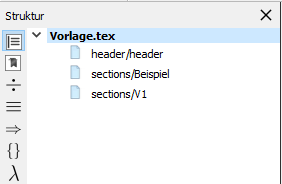
\includegraphics[height=5cm]{images/docstrukt}
%	\captionof{figure}{Struktur Vorlage}
%	\label{fig:docstruct}
%\end{minipage}\hspace{3cm}
%\begin{minipage}[h]{6cm}
%	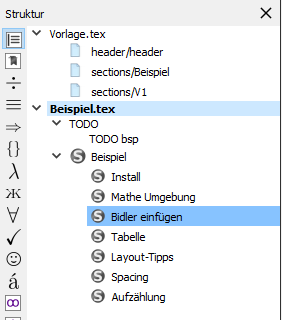
\includegraphics[height=5cm]{images/bspstruct}
%	\captionof{figure}{Struktur Beispiel}
%	\label{fig:bspstruct}
%\end{minipage}
%\\\\\\
%Die in diesem Kapitel behandelten Features sind für diesen Kurs ausreichen.\\
Für eine detailliertere Einführung in \texstud : \href{http://www.mi.uni-koeln.de/wp-MIEDV/wp-content/uploads/2016/05/dokumentNeuYP.pdf}{{\color{blue}\texstud -Einführung}}